\documentclass[../../main.tex]{subfiles}

 \lhead{Implementation: Software}
 
\begin{document}

	\subsection{Software}
		
		%Overall idea
		As a software patch was already in use with the \ac{VSS}, the idea was to extend this software patch to accommodate the newly proposed functionality.

		The software implementation was split into two main sections: \textbf{Location Selection} and \textbf{Mobility}.

		\subsubsection{Location Selection}
			%User interface section
			%The location selection part of the system was required to present the user with an interface with which they could select a location within the \ac{VAE}. The system would then interpret their input and select the correct \ac{RIR} file(s) to be used in the rest of the system. 

			In order to allow the user to move themselves around the room, they had to be presented with a means of doing so. This involved presenting the user with an interface that resembled the space available to them on which they could select their location. This then had to output the coordinates selected by the user and convert them into a format which can be interpreted as a file name which involve 001 - 240. This could then be passed to the rest of the system to load appropriate files. A simple block diagram of the user interface part of the system is shown in figure~\ref{flowDiagram}.


			%-------------Max UI Flow diagram-------------%
			\begin{figure}[H]
				\centerline{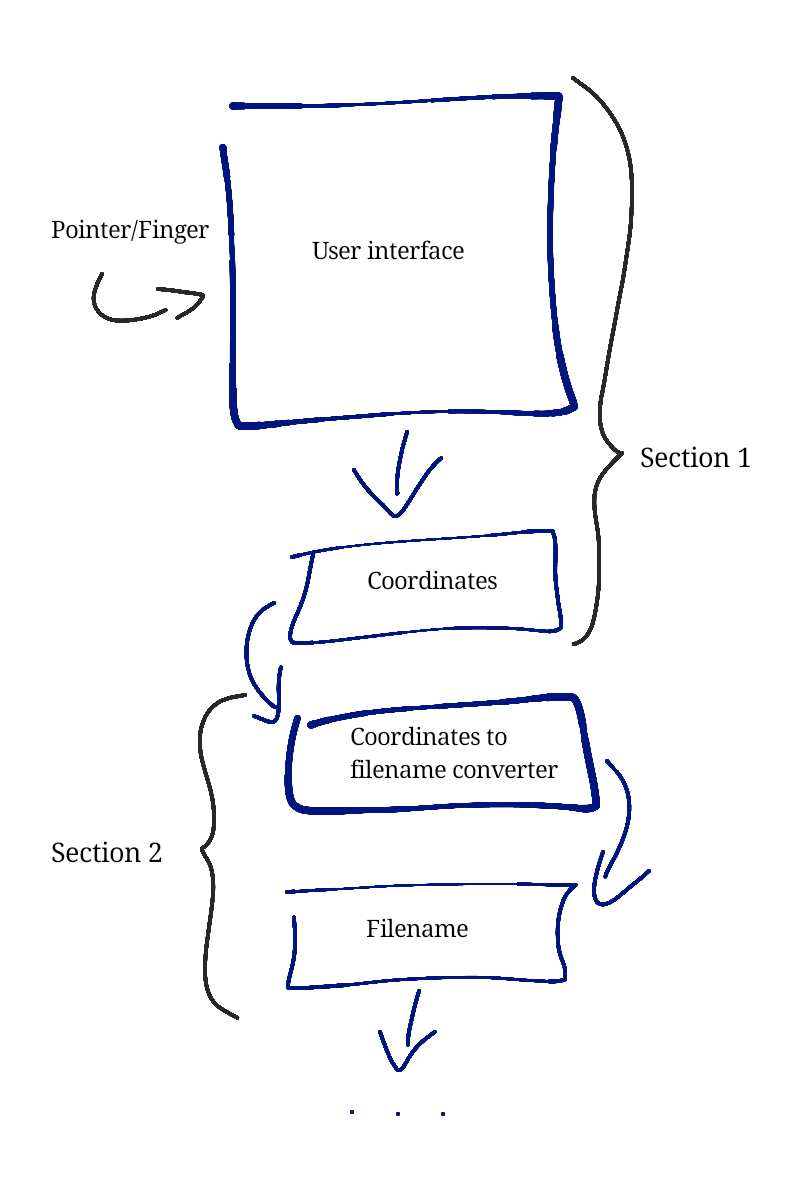
\includegraphics[scale = 0.3]{Sections/Implementation/Max/images/FlowDiagrams/Max1_V2.png}}
				\caption{Flow diagram of the location selection software design}
				\label{flowDiagram}
			\end{figure}

			In Max, the ‘lcd’ object is used for this function. This object presents a quadrilateral of variable length and height with the ability to output its dimensional information by sending a ‘getSize’ message to its input, as well as output the coordinates of a mouse click/drag. Figure~\ref{lcd} shows the lcd object with its inputs and outputs represented by section 1 in the flow diagram.

			%-------------LCD Image-------------%
			\begin{figure}[H]
				\centerline{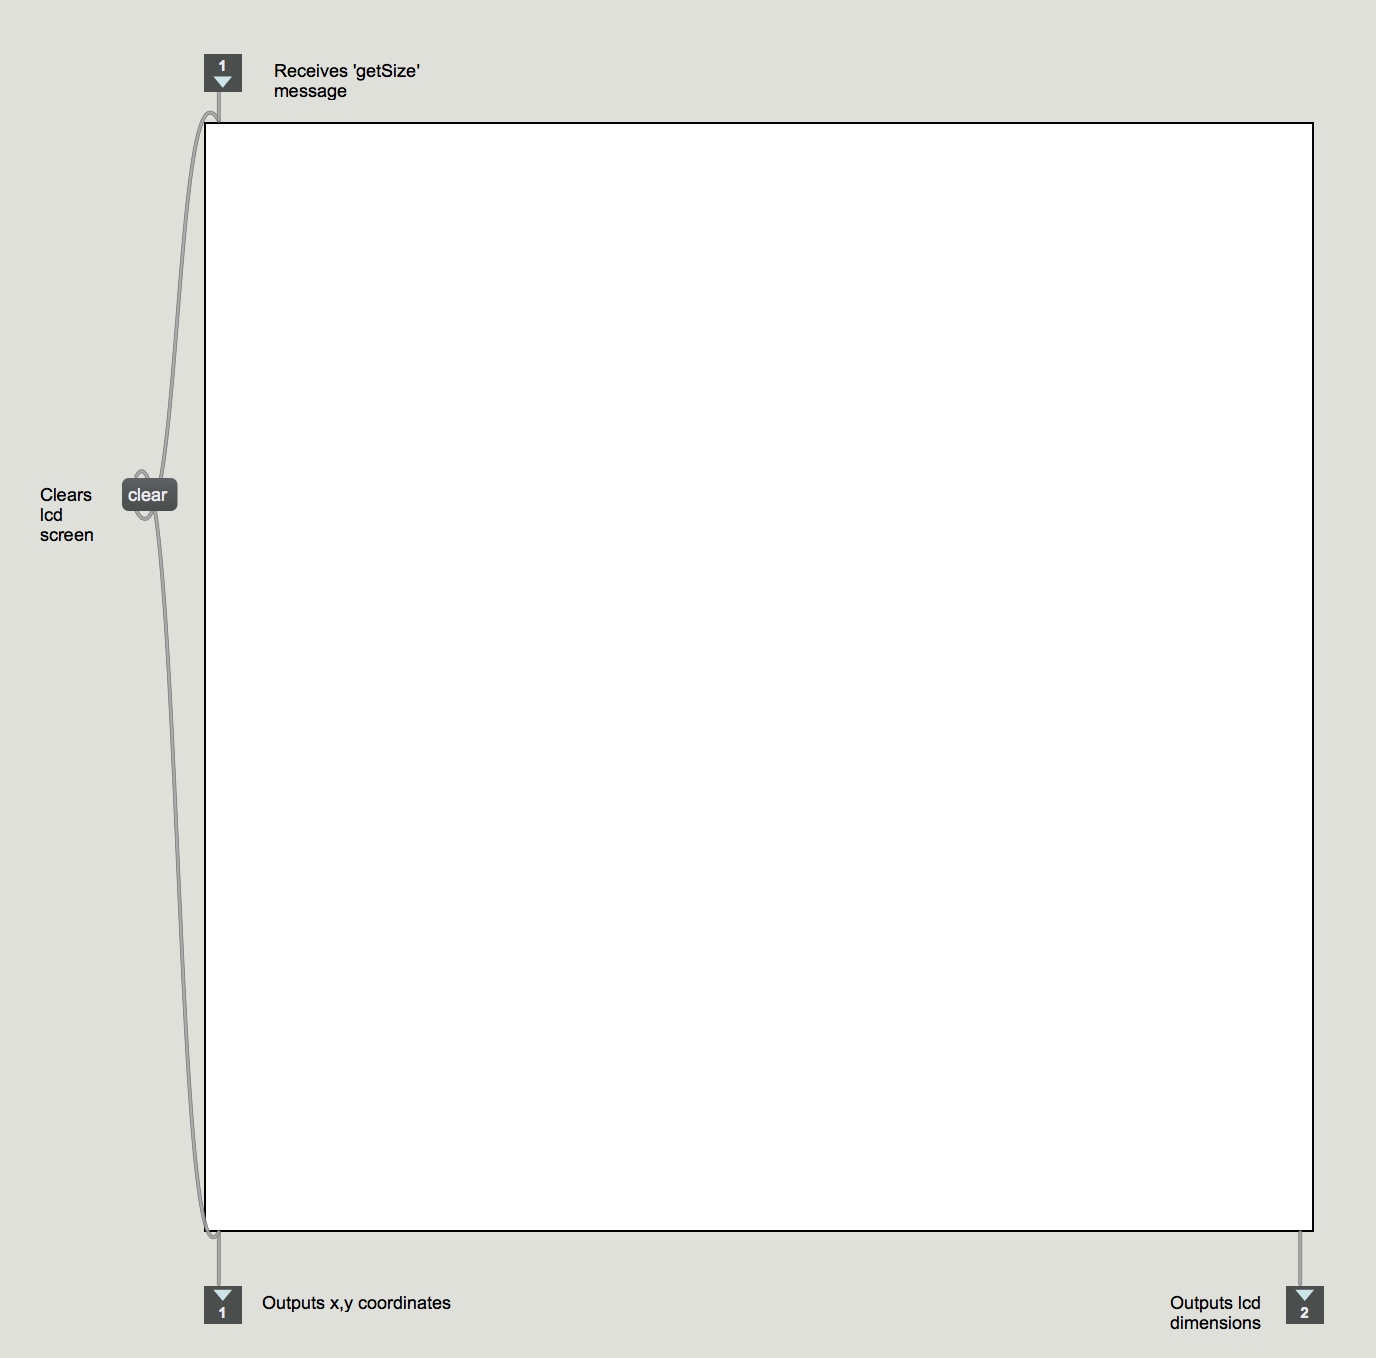
\includegraphics[scale = 0.4]{Sections/Implementation/Max/images/Max/lcd.png}}
				\caption{Flow diagram of the location selection software design}
				\label{lcd}
			\end{figure}

			The outputs from the lcd object are sent to the patch ‘UI_to_file’ which contains a JavaScript file called ‘loadFilesLogic’. This file converts the (x,y) coordinates into an appropriate filename, by taking into account the size of the lcd screen and how many RIRs there are per meter. 

			%-------------LCD Image-------------%
			\begin{figure}[H]
				\centerline{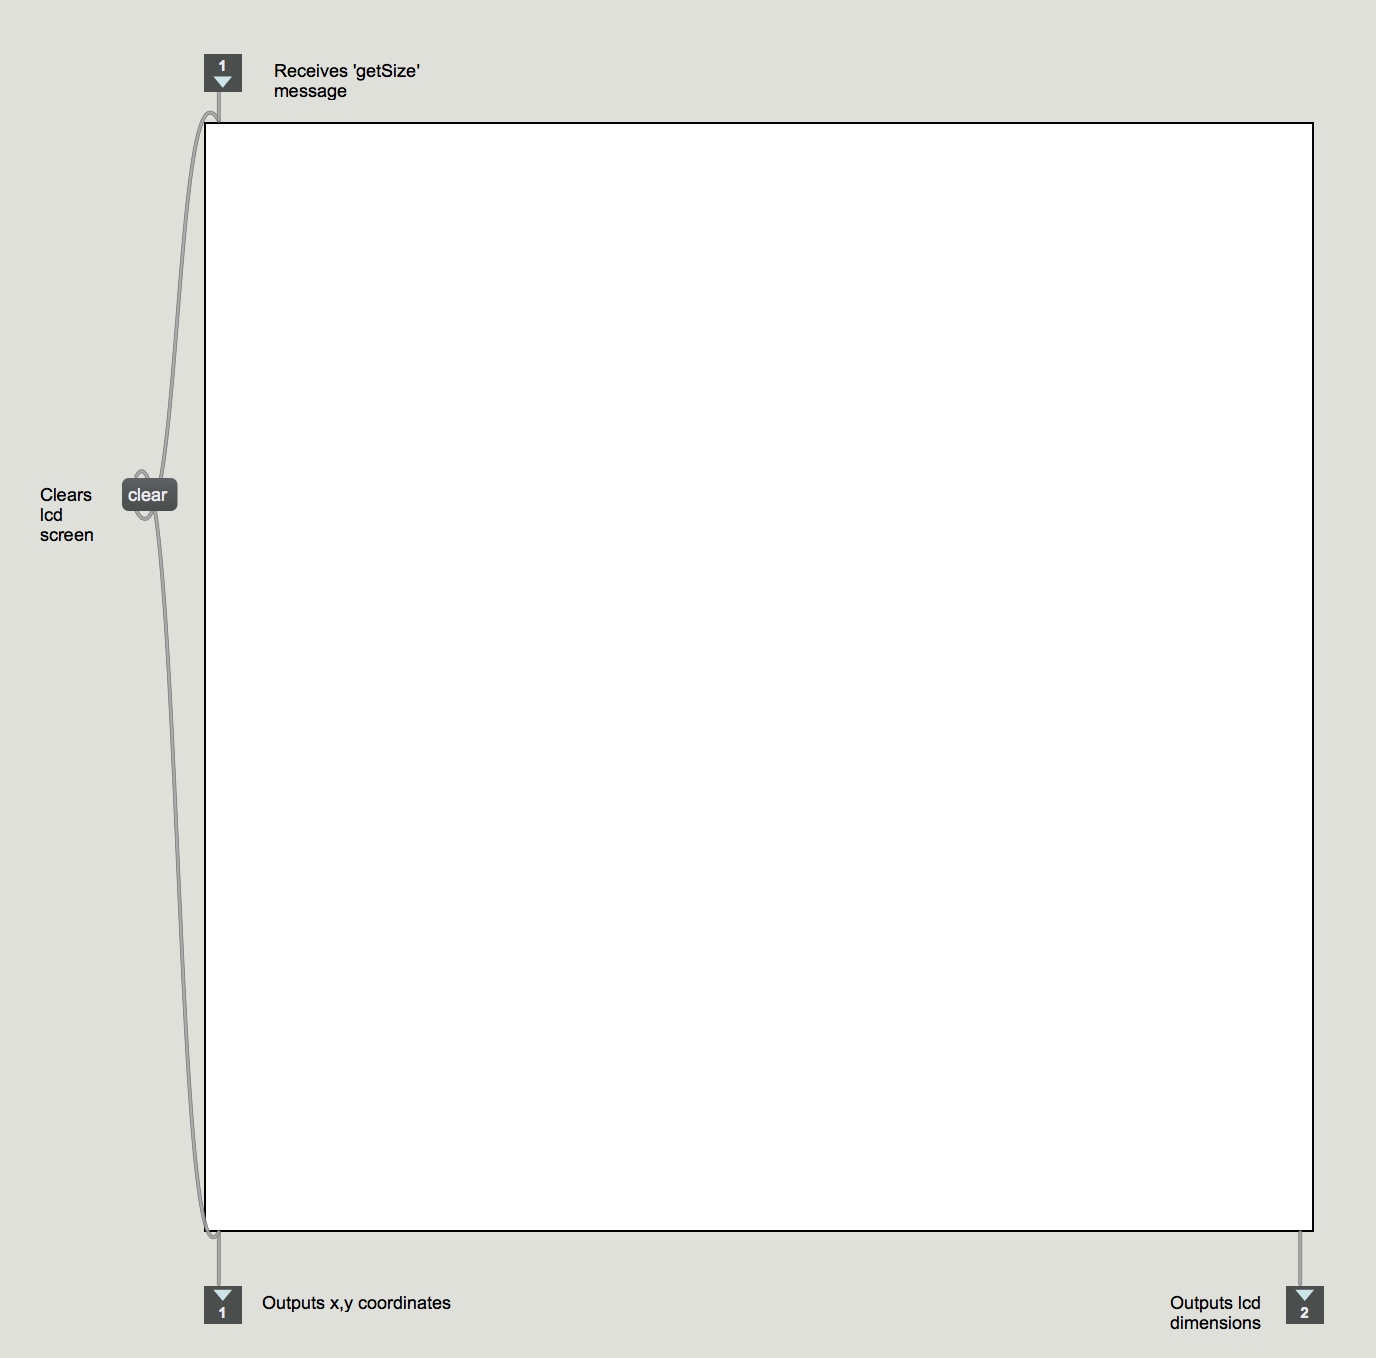
\includegraphics[scale = 0.4]{Sections/Implementation/Max/images/Max/lcd.png}}
				\caption{Flow diagram of the location selection software design}
				\label{lcd}
			\end{figure}


		\subsubsection{Mobility Implementation}

		 \paragraph{Iteration 1}
		 	%Idea to stay between RIRs in a grid

		 	%Loading issued

		 \paragraph{Iteration 2}
		 	%Preload RIRs

		 \paragraph{Iteration 3}
		 	%Path defining



	\subsection{Head-Tracking}
		YEI Sensor was not good.


	\subsection{Latency Test}
	
	\subsection{RIR Trimming}

\end{document}